%%{\Large Quem duvida da duvida tem culpa, quem evita a duvida também tem}.
%\begin{center}
%%	{	\huge if (u == !slackware)
%%	
%%		{u == !hacker}}
%	
%	
\includegraphics[width=.4\linewidth]{./IMG-GIT/digital-pirate-thumbnail-black.png}
%	
%	
%%	{\huge Just 4t Luzl}
%\end{center}
%
%\vfill\null\columnbreak
%
%{\LARGE @aravecchia3d}
%
%\begin{itemize}
%	\item mago do 3D,
%	\item guerreiro do software livre,
%	\item o 3\textordmasculine\space de sua casa
%	\item e o 1\textordmasculine\space de seu nome;
%	\item mestre do Arduino,
%	\item catequizador Linux,
%	\item nascido do terminal,
%	\item batizado em /bin/bash,
%	\item e forjado no Slackware.
%	\item (fiz alguma coisa errada?)
%\end{itemize}
%
%\vfill \null \columnbreak
%
{
%	\pagecolor{black}

\begin{center}
	
\includegraphics[width=.7\linewidth]{./IMG-GIT/digital-pirate-thumbnail-black.png}
\end{center}

	\begin{center}
	{\Huge H4CK3R}
\end{center}
\vfill\null
\columnbreak

\huge
\begin{itemize}
	\item Alfabeto 1337:
	
	\LARGE
	\begin{itemize}
		\item Como não ser kickado no IRC.
		\item BAN te conhecer.
	\end{itemize}
\end{itemize}

\begin{center}
	\Huge 4 B C D 3 F 6 H 1 J K L M N 0 P Q R 5 7 U V W X Y Z
	
	\vfill\null
	\columnbreak
		
	{\LARGE	
		\vspace*{20mm}
		P1R4T4
		
		A = 01000001\\$ \neq $\\4 = 00110100
	}
\end{center}
}
\vfill\null
\columnbreak

%\textbf 

\huge

 \href{https://en.wikipedia.org/wiki/Alan_Turing}{Alan Turing}

%{\Large \href{https://l.facebook.com/l.php?u=https\%3A\%2F\%2Fwww.estadao.com.br\%2Finternacional\%2Fcomo-a-finlandia-usou-as-salas-de-aula-para-derrotar-as-fake-news\%2F\%3Ffbclid\%3DIwAR3IrcYDLX6Ssz9qyvYaiK3Y98knk3IlmM_7TjRB_TDlBacY_KlOqMToSZs&h=AT2rFZTJ4u_rhbWxDWTfZ9BdadL5xvTJxEMilcoN8Ive9qvT9Lnu2Xa5F_chD-ZG_cq6NL8W9_C6bZNJfOgzcwrsXmMlBd2VtYUh7BL9ETPn6IZJffz21KaaKRVWFPw1kmRXIVK_RjGc&__tn__=R*F&c[0]=AT0X9bA0Yfw96qGCeQk1gw-YpCb1sOF7edG7lQ-UrlFMswYITGRspRCXbO8LOZBiW6jgYPdh-gkIsF3ZS3lj-zfHrcWUJbD3vQPlUxjHm-xefKAkF2Dsy2-bumgoP52m8LZKUFsUx9xjI4UBXWjEruJ9tPrEOFqdYnCY3-1tdafepOs1Dx_p2hJqqE1a04Kb1yK1u9KYD2s2mPFvWOlL-x1wPyQ8ViXLhKINeb2ooD0kKIXsOQ}{Alan Turing}}


\begin{center}
	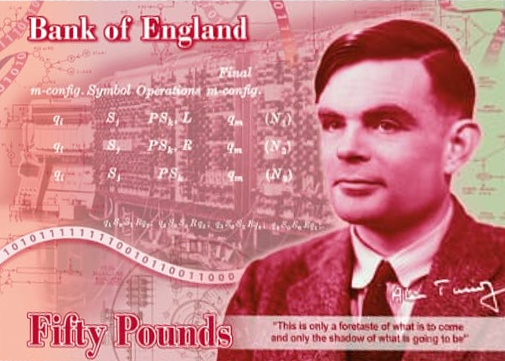
\includegraphics[width=.8\linewidth]{./IMG-GIT/turing-note.jpeg}
\end{center}

\vfill\null
\columnbreak

{\Large
	\begin{itemize}
		\item  Cavalheiro da Inglaterra
		\item Herói da 2\textordfeminine\space Guerra Mundial
		\item Pai da Ciência da Computação
		\item Pai de todos os hackers.
	\end{itemize}
}

\vfill\null
\columnbreak

\begin{center}
		\href{https://pt.wikipedia.org/wiki/Colossus_(computador)}{Colossus}

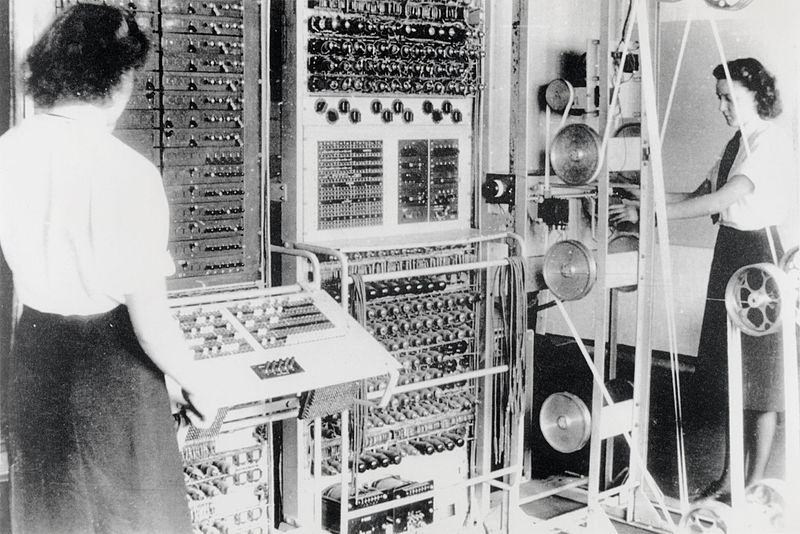
\includegraphics[width=.8\columnwidth]{./IMG-GIT/CIENTISTAS/Colossus.jpg}

\vfill\null
\columnbreak		

\href{https://pt.wikipedia.org/wiki/Enigma_(m\%C3\%A1quina)}{Enigma?}

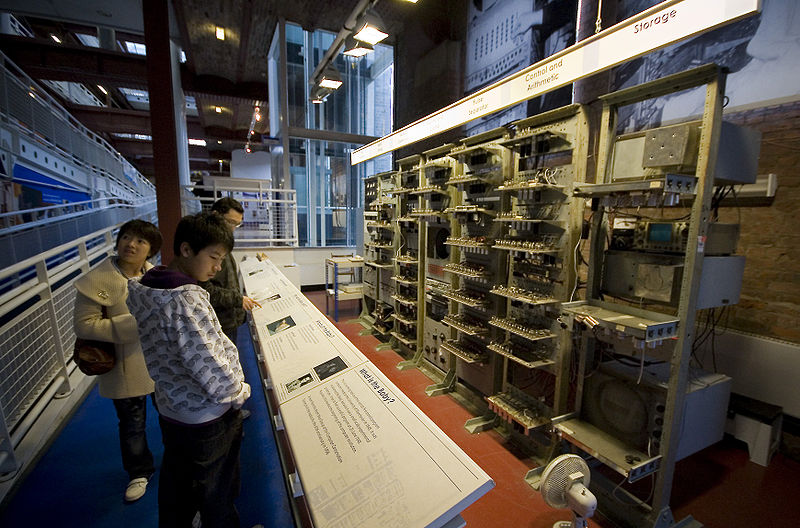
\includegraphics[width=.8\columnwidth]{./IMG-GIT/CIENTISTAS/800px-SSEM_Manchester_museum.jpg}

\vfill\null
\columnbreak	

\href{https://pt.wikipedia.org/wiki/M\%C3\%A1quina_de_Turing}{Maquina de Turing}


\includegraphics[width=\linewidth]{./IMG-GIT/CIENTISTAS/300px-Turing_Machine.png}

\vfill\null
\pagebreak	

\href{https://pt.wikipedia.org/wiki/M\%C3\%A1quina_de_Turing}{Maquina de Turing}


\includegraphics[height=.8\textheight]{./IMG-GIT/CIENTISTAS/300px-Turing_Machine.png}


\end{center}

\vfill\null
\pagebreak

\LARGE \href{https://pt.wikipedia.org/wiki/Steve_Jobs}{Steve Jobs}
	
		\begin{center}
		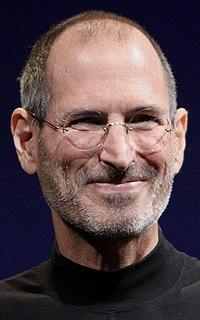
\includegraphics[height=.7\textheight]{./IMG-GIT/jobs.jpg}
	\end{center}
%width=.8\columnwidth

\vfill\null
\columnbreak

\href{https://pt.wikipedia.org/wiki/Steve_Wozniak}{Steve Wozniak}

	\begin{center}
		
\includegraphics[height=.7\textheight]{./IMG-GIT/woz.jpg}
	\end{center}
	
\vfill\null
\pagebreak



\LARGE

\begin{multicols}{3}


	\begin{center}
		\href{https://pt.wikipedia.org/wiki/Bill_Gates}{Bill\\ Gates}
		
		
\includegraphics[width=.8\columnwidth]{./IMG-GIT/bill.jpg}
	\end{center}

\vfill\null
\columnbreak

	\begin{center}
		\href{https://pt.wikipedia.org/wiki/Richard_Matthew_Stallman}{Richard Matthew Stallman \\(RMS)}
		
		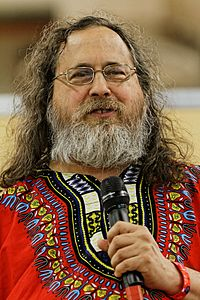
\includegraphics[width=.7\columnwidth]{./IMG-GIT/rms.jpg}
	\end{center}

\vfill
\columnbreak

\begin{center}
	\href{https://pt.wikipedia.org/wiki/Linus_Torvalds}{Linus \\Torvalds}
	
	\includegraphics[width=.8\columnwidth]{./IMG-GIT/linus.jpeg}
\end{center}

\vfill\null
\pagebreak				

\href{https://pt.wikipedia.org/wiki/Dennis_Ritchie}{Dennis Ritchie}

\href{https://pt.wikipedia.org/wiki/Ken_Thompson}{Ken Thompson}

%\href{https://pt.wikipedia.org/wiki/Linguagem_de_programa\%C3\%A7\%C3\%A3o}{linguagem de programação}

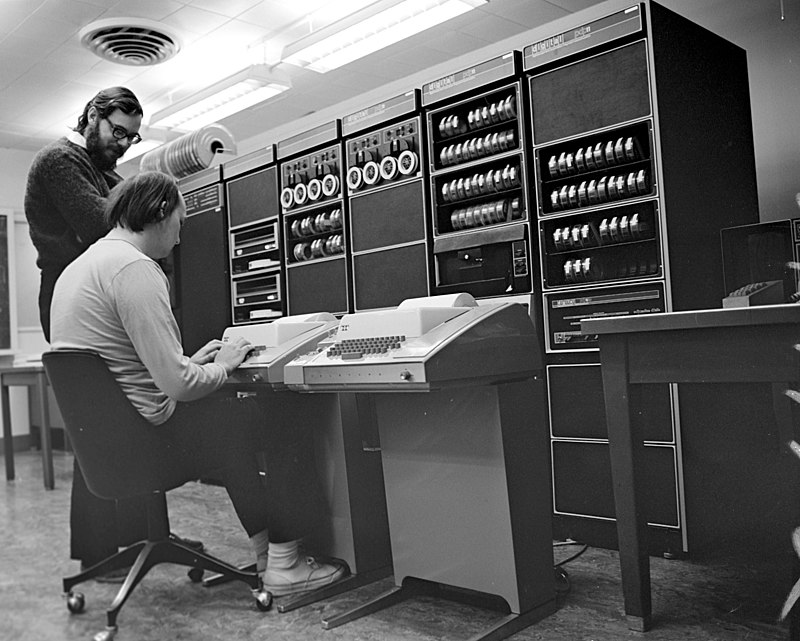
\includegraphics[width=.8\linewidth]{./IMG-GIT/CIENTISTAS/Ken_Thompson_(sitting)_and_Dennis_Ritchie_at_PDP-11_(2876612463).jpg}

\vfill
\columnbreak

\href{https://pt.wikipedia.org/wiki/Linguagem_de_programa\%C3\%A7\%C3\%A3o}{Linguagens de programação}

\begin{itemize}
	\item Unix
	\item B (linguagem de programação)
	\item C (linguagem de programação)
	\item UTF-8
	\item Tabelas de finais (enxadrismo)
\end{itemize}
\end{multicols}

\vfill\null
\pagebreak

\begin{multicols}{2}
	\begin{quote}
	``O homem só chegou na Lua porque era um computador que estava pilotando a nave.'' \\
\begin{flushright}
		\textit{Autor Desconhecido}
\end{flushright}
\end{quote}

\vfill
\columnbreak

\begin{quote}
	``A necessidade é a mãe de todas as invenções.'' \\
	\begin{flushright}
		\textit{Platão}
	\end{flushright}
\end{quote}
\end{multicols}


\vfill\null
\pagebreak	


\begin{multicols}{4}[Outros nomes importantes:]
	\href{https://pt.wikipedia.org/wiki/Blaise_Pascal}{Blaise Pascal}
	
\begin{center}
		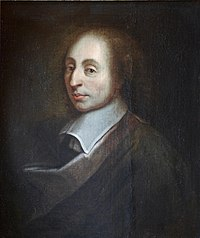
\includegraphics[width=.8\columnwidth]{./IMG-GIT/CIENTISTAS/Blaise_Pascal_Versailles.JPG}
\end{center}

\vfill\null
\columnbreak

\begin{center}
	\href{https://pt.wikipedia.org/wiki/Charles_Babbage}{Charles Babbage}


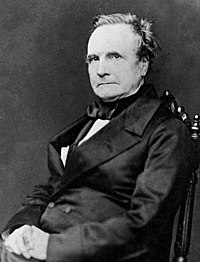
\includegraphics[width=.8\columnwidth]{./IMG-GIT/CIENTISTAS/Charles_Babbage_-_1860.jpg}
\end{center}

\vfill\null
\columnbreak

\href{https://pt.wikipedia.org/wiki/Ada_Lovelace}{Ada Lovelace}

\begin{center}
	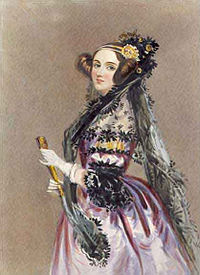
\includegraphics[width=.8\columnwidth]{./IMG-GIT/CIENTISTAS/200px-Ada_lovelace.jpg}
\end{center}

\vfill\null
\columnbreak

\href{https://pt.wikipedia.org/wiki/George_Boole}{George Boole}

\begin{center}
	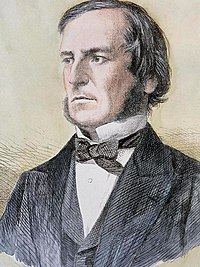
\includegraphics[width=.8\columnwidth]{./IMG-GIT/CIENTISTAS/200px-George_Boole_color.jpg}
\end{center}

\vfill\null
\columnbreak
	
		
			\href{https://pt.wikipedia.org/wiki/John_von_Neumann}{John von Neumann}
			
\begin{center}
				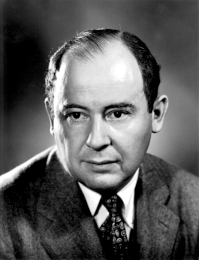
\includegraphics[width=.8\columnwidth]{./IMG-GIT/CIENTISTAS/JohnvonNeumann-LosAlamos.jpg}
\end{center}
			
\vfill\null
\columnbreak			
			
			\href{https://pt.wikipedia.org/wiki/Mem\%C3\%B3ria_de_computador}{memória}
			
\begin{center}
				\includegraphics[width=.8\columnwidth]{./IMG-GIT/CIENTISTAS/linus.jpeg}
\end{center}
			
			\vfill\null
			\pagebreak	
			
			\href{https://pt.wikipedia.org/wiki/M\%C3\%A1quina_de_Turing}{Maquina de Turing}
			
			
\includegraphics[height=.8\textheight]{./IMG-GIT/CIENTISTAS/300px-Turing_Machine.png}
			
\vfill\null
\pagebreak
			
				    \href{https://pt.wikipedia.org/wiki/Arquitetura_de_von_Neumann}{Arquitetura de von Neumann}

\begin{center}
	\includegraphics[width=.8\columnwidth]{./IMG-GIT/CIENTISTAS/linus.jpeg}
\end{center}
				    
\vfill\null
\columnbreak				    
				    
				\href{https://pt.wikipedia.org/wiki/John_Backus}{John Backus}
				
\begin{center}
					\includegraphics[width=.8\columnwidth]{./IMG-GIT/CIENTISTAS/linus.jpeg}
\end{center}
				
\vfill\null
\columnbreak				
				
				\href{https://pt.wikipedia.org/wiki/Fortran}{Fortran}
				
\begin{center}
					\includegraphics[width=.8\columnwidth]{./IMG-GIT/CIENTISTAS/linus.jpeg}
\end{center}
				
\vfill\null
\columnbreak				
				
				\href{https://pt.wikipedia.org/wiki/BNF}{BNF}
				
\begin{center}
					\includegraphics[width=.8\columnwidth]{./IMG-GIT/CIENTISTAS/linus.jpeg}
\end{center}
				
\vfill\null
\columnbreak				
				
				\href{https://pt.wikipedia.org/wiki/Maurice_V._Wilkes}{Maurice V. Wilkes}
				
\begin{center}
					\includegraphics[width=.8\columnwidth]{./IMG-GIT/CIENTISTAS/linus.jpeg}
\end{center}
				
\vfill\null
\columnbreak				
				
				\href{https://pt.wikipedia.org/wiki/Howard_Aiken}{Howard Aiken}
				
\begin{center}
					\includegraphics[width=.8\columnwidth]{./IMG-GIT/CIENTISTAS/linus.jpeg}
\end{center}
				
\vfill\null
\columnbreak				
				
				\href{https://pt.wikipedia.org/wiki/Mark_I}{Mark I}
				
\begin{center}
					\includegraphics[width=.8\columnwidth]{./IMG-GIT/CIENTISTAS/linus.jpeg}
\end{center}
				
\vfill\null
\columnbreak				
				
				\href{https://pt.wikipedia.org/wiki/Walter_H._Brattain}{Walter H. Brattain}
				
\begin{center}
					\includegraphics[width=.8\columnwidth]{./IMG-GIT/CIENTISTAS/linus.jpeg}
\end{center}
				
\vfill\null
\columnbreak				
				
				\href{https://pt.wikipedia.org/wiki/John_Presper_Eckert}{John Presper Eckert}
				
\begin{center}
					\includegraphics[width=.8\columnwidth]{./IMG-GIT/CIENTISTAS/linus.jpeg}
\end{center}
				
\vfill\null
\columnbreak				
				
				\href{https://pt.wikipedia.org/wiki/William_Shockley}{William Shockley}
				
\begin{center}
					\includegraphics[width=.8\columnwidth]{./IMG-GIT/CIENTISTAS/linus.jpeg}
\end{center}
				
\vfill\null
\columnbreak				
				
				\href{https://pt.wikipedia.org/wiki/Robert_Noyce}{Robert Noyce}
				
\begin{center}
					\includegraphics[width=.8\columnwidth]{./IMG-GIT/CIENTISTAS/linus.jpeg}
\end{center}
				
\vfill\null
\columnbreak				
				
				\href{https://pt.wikipedia.org/wiki/Gordon_Moore}{Gordon Moore}
				
\begin{center}
					\includegraphics[width=.8\columnwidth]{./IMG-GIT/CIENTISTAS/linus.jpeg}
\end{center}
				
\vfill\null
\columnbreak				
				
				\href{https://pt.wikipedia.org/wiki/Richard_Hamming}{Richard Hamming}
				
\begin{center}
					\includegraphics[width=.8\columnwidth]{./IMG-GIT/CIENTISTAS/linus.jpeg}
\end{center}
				
\vfill\null
\columnbreak				
				
				\href{https://pt.wikipedia.org/wiki/Grace_Hopper}{Grace Hopper}
				
\begin{center}
					\includegraphics[width=.8\columnwidth]{./IMG-GIT/CIENTISTAS/linus.jpeg}
\end{center}
				
\vfill\null
\columnbreak				
				
				\href{https://pt.wikipedia.org/wiki/Jean_I._Bach}{Jean I. Bach}
				
\begin{center}
					\includegraphics[width=.8\columnwidth]{./IMG-GIT/CIENTISTAS/linus.jpeg}
\end{center}
				
\vfill\null
\columnbreak				
				
				\href{https://pt.wikipedia.org/wiki/E._F._Codd}{E. F. Codd}
				
\begin{center}
					\includegraphics[width=.8\columnwidth]{./IMG-GIT/CIENTISTAS/linus.jpeg}
\end{center}
				
\vfill\null
\columnbreak				
				
				\href{https://pt.wikipedia.org/wiki/Stephen_Cook}{Stephen Cook}
				
\begin{center}
					\includegraphics[width=.8\columnwidth]{./IMG-GIT/CIENTISTAS/linus.jpeg}
\end{center}
				
\vfill\null
\columnbreak				
				
				\href{https://pt.wikipedia.org/wiki/Michael_O._Rabin}{Michael O. Rabin}
				
\begin{center}
					\includegraphics[width=.8\columnwidth]{./IMG-GIT/CIENTISTAS/linus.jpeg}
\end{center}
				
\vfill\null
\columnbreak				
				
				\href{https://pt.wikipedia.org/wiki/Robert_Tarjan}{Robert Tarjan}
				
\begin{center}
					\includegraphics[width=.8\columnwidth]{./IMG-GIT/CIENTISTAS/linus.jpeg}
\end{center}
				
\vfill\null
\columnbreak				
				
				\href{https://pt.wikipedia.org/wiki/Leslie_Lamport}{Leslie Lamport}
				
\begin{center}
					\includegraphics[width=.8\columnwidth]{./IMG-GIT/CIENTISTAS/linus.jpeg}
\end{center}
				
\vfill\null
\columnbreak				
				
				\href{https://pt.wikipedia.org/wiki/Adi_Shamir}{Adi Shamir}
				
\begin{center}
					\includegraphics[width=.8\columnwidth]{./IMG-GIT/CIENTISTAS/linus.jpeg}
\end{center}
				
\vfill\null
\columnbreak				
				
				\href{https://pt.wikipedia.org/wiki/Ronald_L._Rivest}{Ronald L. Rivest}
				
\begin{center}
					\includegraphics[width=.8\columnwidth]{./IMG-GIT/CIENTISTAS/linus.jpeg}
\end{center}
				
\vfill\null
\columnbreak				
				
				\href{https://pt.wikipedia.org/wiki/Leonard_Adleman}{Leonard Adleman}
				
\begin{center}
					\includegraphics[width=.8\columnwidth]{./IMG-GIT/CIENTISTAS/linus.jpeg}
\end{center}
				
\vfill\null
\columnbreak				
				
				\href{https://pt.wikipedia.org/wiki/Whitfield_Diffie}{Whitfield Diffie}
				
\begin{center}
					\includegraphics[width=.8\columnwidth]{./IMG-GIT/CIENTISTAS/linus.jpeg}
\end{center}
				
\vfill\null
\columnbreak				
				
				\href{https://pt.wikipedia.org/wiki/Martin_Hellman}{Martin Hellman}
				
\begin{center}
					\includegraphics[width=.8\columnwidth]{./IMG-GIT/CIENTISTAS/linus.jpeg}
\end{center}
				
\vfill\null

\columnbreak				
				
				\href{https://pt.wikipedia.org/wiki/Ronald_L._Rivest}{Ronald L. Rivest}
				
\begin{center}
					\includegraphics[width=.8\columnwidth]{./IMG-GIT/CIENTISTAS/linus.jpeg}
\end{center}
				
\vfill\null

\columnbreak				
				
				\href{https://pt.wikipedia.org/wiki/Adi_Shamir}{Adi Shamir}
				
\begin{center}
					\includegraphics[width=.8\columnwidth]{./IMG-GIT/CIENTISTAS/linus.jpeg}
\end{center}
				
\vfill\null

\columnbreak				
				
				\href{https://pt.wikipedia.org/wiki/Leonard_Adleman}{Leonard Adleman}
				
\begin{center}
					\includegraphics[width=.8\columnwidth]{./IMG-GIT/CIENTISTAS/linus.jpeg}
\end{center}
				
\vfill\null

\columnbreak				
				
				\href{https://pt.wikipedia.org/wiki/Jim_Gray}{Jim Gray}
				
\begin{center}
					\includegraphics[width=.8\columnwidth]{./IMG-GIT/CIENTISTAS/linus.jpeg}
\end{center}
				
\vfill\null

\columnbreak				
				
				\href{https://pt.wikipedia.org/wiki/Michael_Stonebraker}{Michael Stonebraker}
				
\begin{center}
					\includegraphics[width=.8\columnwidth]{./IMG-GIT/CIENTISTAS/linus.jpeg}
\end{center}
				
\vfill\null

\pagebreak
				
\end{multicols}
\begin{multicols}{2}
	
	\Large
\begin{itemize}
	\item \textbf{Falso}: o Hacker no cinema e na televisão.
\begin{itemize}
	\item Hacker não e aquele que invade computadores, o nome disso é \textbf{criminoso}, mesmo.
	\item Hacking não é sobre invadir computadores, e sobre construí-los.
\end{itemize}
	\item \textbf{Verdadeiro}: a grande maioria dos \textbf{hackers de verdade} não sabe invadir nem o wifi do vizinho, e não esta nem interessado em aprender!
	\item Estao ocupados demais:
	\begin{enumerate}
		\item Ganhando dinheiro.
		\item Salvando o mundo.
		\item Colocando mais computadores nas escolas.
		\begin{enumerate}
			\item Estudando.
			\item Trabalhando.
			\item Se divertindo!
			\item Construindo robôs.
			\item Escrevendo programas mais seguros (incluindo video-games).
			\item Monitorando chuvas, tempestades, terremotos e pandemias.
			\item Mandando naves e satelites para outros planetas.
			\item 		Combatendo o Covid: \href{https://brasil.io/covid19/}{ (Hack the world!)}
			\item Tentando achar a cura para o câncer.
			\item Ensinando computação para crianças nas escolas.
			\item Cuidando da segurança de escolas, bancos, empresas, policia, exército...
		\end{enumerate}
	\end{enumerate}
\end{itemize}
\begin{enumerate}
	
	\item História da 2\textordfeminine\space Guerra Mundial.
	\item Nazismo: o inimigo do meu inimigo é meu amigo. Quando capitalistas e comunistas lutaram do mesmo lado.
	\item Holocausto.
	\item Guerras alavancam a tecnologia.
	\item \href{https://pt.wikipedia.org/wiki/Enigma\_(m%C3%A1quina)}{A máquina Enigma}.
	\item A única forma de vencer uma máquina. inteligente e utilizando outra mais inteligente.
	\item \href{https://youtu.be/mwFWMM9APLs?t=170}{O jogo da Imitação}.
	\item A bomba atômica.
	\item ENIAC.
	\item Os primeiros computadores militares.
	\item ARPANET.
	\item Milnet e Internet.
	\item Os primeiros Mainframes.
	\item Um inseto.
	\item Origem da palavra Hacker.
	\item Hackers hoje.
	\begin{enumerate}
		\item Gurus
		\item Cybersec Hackers
		\item Eletronic Hackers, os caras do baixo nível.
		\item White hats.
		\item Black hats.
		\item Gray hats.
		\item Red Hat.
		\item U can't HACK if U don't SLACK.
		\item BackTrack, Kali e distribuições especializadas.
		\item Programadores e outros Hackers.
\item
	\end{enumerate}
\end{enumerate}

\end{multicols}